\documentclass[../../../main]{subfiles}


\begin{document}

\section{Microcontroller implementation}

This section as the purpose of detailing how the software for the Tiva microcontroller is setup and why. The responsibility of the Tiva is to act as the brain of the entire system while the FPGA acts like a data acquisitions device and a hardware controller. 

The operating system used as the platform on the Tiva is FreeRTOS, an open source RealTime operating system created by Real Time Engineers LTD.

FreeRTOS handles system processes of different types by creating "Tasks" that are the run using a preemptive scheduler which allows the system to not only run multiple tasks in "parallel"\footnote{Due to only one core being supported, true parallel is not possible.} but also efficiently allocate the systems resources available.


A task is a single area of responsibility that either by necessity or by convention is combined as a single logical unit. Each task in the system (a full overview can be seen in the task diagram) can then be scheduled based on the priority it has been assigned and whether the task itself has decided that it wants to be scheduled. 

\section{Scheduling}

In order to enable the microcontroller to run more then one task some form of scheduling must be implemented. This allows the operating system\footnote{FreeRTOS} to make a choice as to what tasks needs processing capacity at this moment in time. In the FreeRTOS based system running on the Tiva scheduling is done trough a priority based preemption\footnote{The ability to pause and resume processes without the process knowing.} capable implementation.

The preemption capability enables the system to respond quickly to higher priority tasks becoming available for execution rather then waiting for the current task to return on its own potentially taking the CPU forever, it will be paused and the higher priority task executed before the lower priority one is resumed and potentially completed.
 
As mentioned the priority allows the system to select more important\footnote{Defined by the programmer} processes to be run quickly when available.  

The schduler is run by a timer interupt every 5ms and during this the current task is paused and the scheduler evaluates the next eleqible task to run, this may be the same task that was running before and this will then be resumed, but the scheduler must be run every 5ms tick.

\section{Subtask Communication}

The multiple task architecture where each task deals only in their own specific area of the system, due to the fact that the tasks need to work together there need to be a way for them to communicate.
This is accomplished using a combination of state buffers and queues. State buffers are simple buffers keeping the last value written to it until a new value is written regardless of reads performed in that time.

All queues in the system are FIFO\footnote{First-In-First-Out} queues allowing easy exchange of data between different parts of the system, while maintaining loose coupling between components. This loose coupling allows more parallel development and a more robust end product. 

To maintain data integrity all shared-write resources are protected with semaphores allowing a task to obtain exclusive access to a resource and be able to update it without risk of data corruption caused by simultaneous access.

\section{Tasks}

The entire system has been created as a task diagram in figure \ref{fig:entire_task_diagram}. 


\begin{itemize}
    \item Describe each task requirements towards the OS
        \begin{itemize}
            \item System tasks
                \begin{itemize}
                    \item Status LED
                    \item UART 
                    \item LCD
                    \item Matrix keyboard
                    \item SPI
                \end{itemize}
                 \item User tasks
                \begin{itemize}
                    \item PID
                    \item User interface
                \end{itemize}
        \end{itemize}
\end{itemize}

\begin{figure}[H]
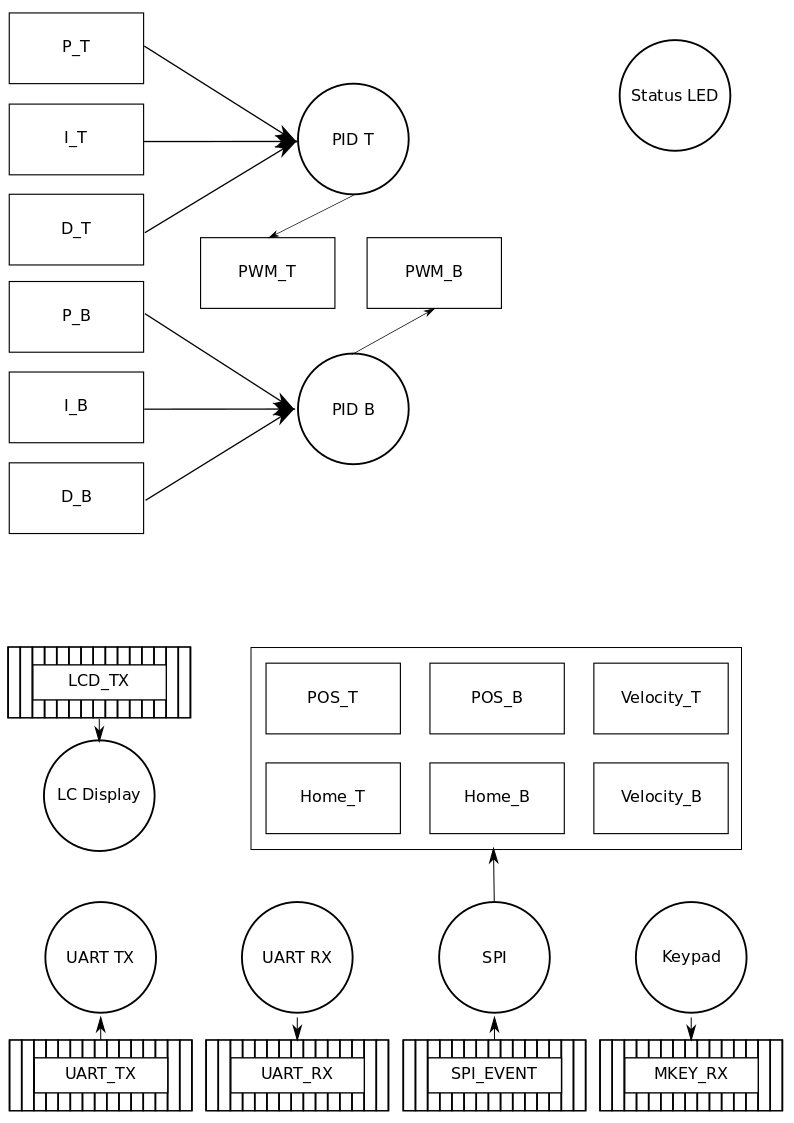
\includegraphics[width=\columnwidth]{taskdiagram_full.png}
\caption{Task Diagram of entire system}
\label{fig:entire_task_diagram}
\end{figure}

\end{document}

